\chapter{Example: Numerical Integration}


%%%%%

In this chapter, we will look at a numerical computing problem that is well
suited to being parallelised, namely to calculate an approximation of a definite
integral:
\[
\int_a^b f(x) \, dx .
\]

%%%%%

\section{The Trapezium Rule}

The trapezium rule is a standard numerical technique to approximate the value
of an integral.  It splits the integral's range $[a,b]$ into $n \ge 1$
intervals:
\[\mstyle
\begin{align}
[{a+i\delta}, a+(i+1)\delta], 
  \quad\mbox{for $i = 0, \ldots, n-1$,} \\
\mbox{where $\delta = (b-a)/n$.}
\end{align}
\]
This is illustrated in Figure~\ref{fig:trapezium} with $n = 4$
(although in practice we would use a much larger value of~$n$).

%%%%%%%%%%%%%%%%

\begin{figure}
\begin{center}
\def\labY{-0.16}
\def\fn{\x^3/240 + \x^2/10 - 0.5*\x + 1.5}   %2.5*\x^2-2*\x+15}
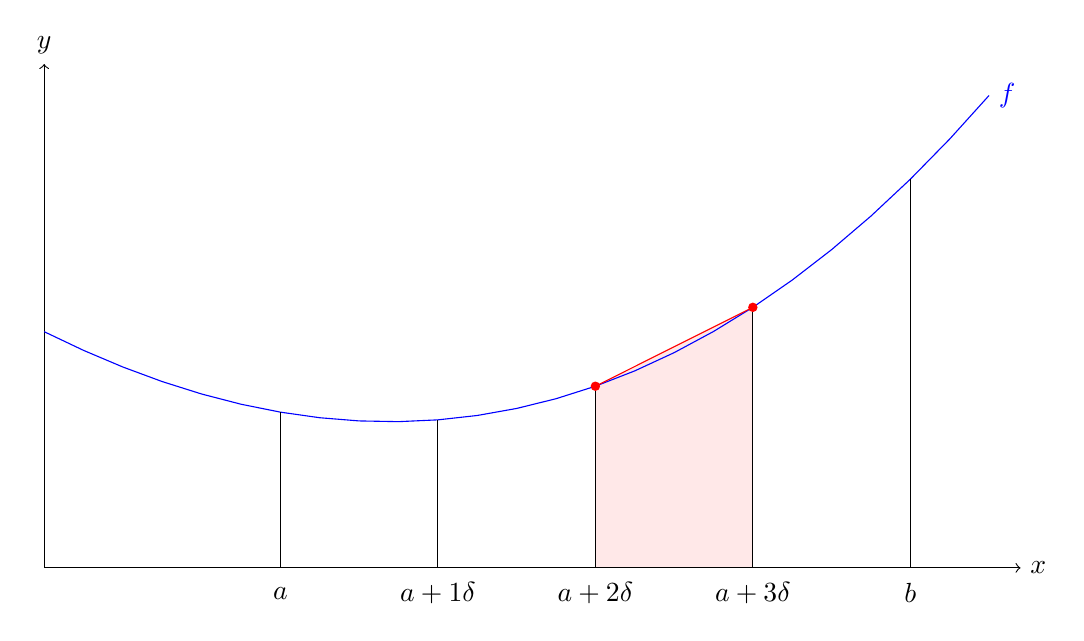
\begin{tikzpicture}[domain=0:6, scale = 2]
% Coordinates of selected points
\foreach \x in {3.5}  \draw (\x,\fn) coordinate (c1); %  node (c1) {};
\foreach \x in {4.5}  \draw (\x,\fn) coordinate (c2) {};
% Fill trapezium
\fill[red!9] (c1) -- (c2) -- (4.5,0) -- (3.5,0) -- (c1);
% Axes
\draw[->] (0,0) -- (6.2,0) node[right] {$x$};
\draw[->] (0,0) -- (0,3.2) node[above] {$y$};
% Plot
\draw[color=blue] plot (\x,\fn) node[right] {$f$}; 
% x labels
\draw(1.5,\labY) node{$a$};
\foreach \x in {1,2,3} \draw (\x+1.5,\labY) node{$a+\x \delta$};
\draw (5.5,\labY) node{$b$};
% Verticals
%\foreach \i in {0,1,2,3,4} \foreach \x in {\i+1.5} 
\foreach \x in {1.5,2.5,3.5,4.5,5.5} 
  \draw (\x,0) -- (\x,\fn);
% Blobs at selected points, and line between them
\draw[red] (c1) -- (c2);
\fill[red] (c1) circle[radius = 0.3mm];
\fill[red] (c2) circle[radius = 0.3mm];
\end{tikzpicture}
\end{center}
\caption{Illustration of the trapezium rule}
\label{fig:trapezium}
\end{figure}

%%%%%

The integral over the interval $[a+i\delta, a+(i+1)\delta]$ can then be
approximated by 
\[\mstyle
\frac{f(a+i\delta)+f(a+(i+1)\delta)}{2} * \delta.
\]
In other words, we approximate the graph of the function over this interval by
a straight line between the endpoints.  This is illustrated in
Figure~\ref{fig:trapezium} for the interval $[a+2\delta, a+3\delta]$.  The red
blobs give the values of the function at the endpoints; the function is
approximated by the red line; and so the integral is approximated by the area
of the pink region.  For this interval, the approach gives a slight
underapproximation. 

Summing over all intervals then gives us the following approximation:
\begin{eqnarray*}
\int_a^b f(x) \, dx  & \approx & 
  \left( \frac{f(a)+f(b)}{2} + \sum_{i=1}^{n-1} f(a+i\delta) \right) * \delta.
\end{eqnarray*}

Figure~\ref{fig:trapezium-sequential} gives straightforward sequential code to
implement the trapezium rule\footnote{The type {\scalashape Double
    \protect\SCALA{=>} Double} represents functions from {\scalashape Double}
  to {\scalashape Double}.}.  (We will see several implementations of the
trapezium rule, so we factor out some common code into an abstract class
|TrapeziumT|.)

%%%%%

\begin{figure}
\begin{scala}
/** Abstract class representing the problem of approximating the integral of £f£
  * from £a£ to £b£. */
abstract class TrapeziumT(f: Double => Double, a: Double, b: Double){
  /** Calculate the integral. */
  def apply(): Double

  /** Use trapezium rule to approximate the integral of £f£ from £left£ to £right£, 
    * using £n£ intervals of size £delta£. 
    * Precondition: £n*delta = right-left£ (modulo rounding errors). */
  protected 
  def integral(left: Double, right: Double, n: Int, delta: Double): Double = {
    require(n > 0 && Math.abs(n*delta-(right-left)) < 0.000000001) 
    var sum: Double=(f(right)+f(left))/2.0
    for(i <- 1 until n) sum += f(left+i*delta)
    sum*delta
  }
}

/** Approximation of the integral of £f£ from £a£ to £b£, using a sequential 
  * implementation of the trapezium rule. */
class SeqTrapezium(f: Double => Double, a: Double, b: Double, n: Int)
    extends TrapeziumT(f, a, b){
  require(n > 0)

  def apply() = integral(a, b, n, (b-a)/n)
}
\end{scala}
\caption{Sequential code to apply the trapezium rule.}
\label{fig:trapezium-sequential}
\end{figure}

%%%%%

\section{A parallel implementation}

Here's the idea of a parallel implementation.  We use some number |nWorkers|
of \emph{worker threads}.  We then split the interval $[a,b]$ into the same
number of equal-size sub-ranges, so each worker works on one sub-range.  A
\emph{controller} thread tells each worker which range to work on.  Each
worker sends its subresult back to the controller, which adds them up to give
the overall result.

This is a form of \emph{data parallelism}.  We split the data (the value
of~$f$ over the relevant range) between the workers.  Each worker calculates a
subresult on its part of the data, and then we combine the subresults. 

%% (This pattern is sometimes known as a \emph{farm}, and the controller as a
%% \emph{farmer}.) 

%%%%%

We will use a channel \SCALA{toWorkers} to communicate from the
controller to the workers, and a channel \SCALA{toController}
to communicate from the workers to the controller.  This is illustrated below.
%
\begin{center}
%\tikzstyle{every node}=[minimum width=5mm,minimum height = 15mm]
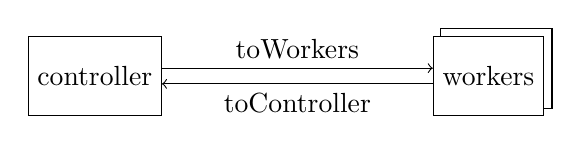
\begin{tikzpicture}
\draw (0,0) node[draw, minimum height = 10mm](c){\scalashape controller};
\draw (5,0) node[draw, minimum height = 10mm] (w){\scalashape workers};
\draw ([xshift = 1mm] w.north west) -- ++ (0,1mm) -- 
  ([xshift = 1mm, yshift = 1mm] w.north east) -- 
  ([xshift = 1mm, yshift = 1mm] w.south east) -- 
  ([yshift = 1mm] w.south east) ;
\draw[->] ([yshift = 1mm] c.east) -- node[above]{\scalashape toWorkers} 
  ([yshift = 1mm] w.west);
\draw[<-] ([yshift = -1mm] c.east) -- node[below]{\scalashape toController} 
  ([yshift = -1mm] w.west);
\end{tikzpicture}
\end{center}

In examples so far, each channel has had one sender and one receiver.
However, an in-port or out-port may be shared between any number of receivers
or senders.  Here, it is useful for the controller to use a single channel to
send to all the workers, and likewise to use a single channel to receive
subresults from all the workers.

Figure~\ref{fig:trapezium-1} gives some of the code.  The companion object
|Trapezium| factors out some definitions that we will reuse in a later
implementation. 

%%%%%

\begin{figure}
\begin{scala}
/** Companion object, collecting some code that is common across 
  * implementations. */
object Trapezium{
  /** Type of tasks to send to client.  The Task £(left, right, taskSize, delta)£
    * represents the task of calculating the integral from £left£ to £right£,
    * using £taskSize£ intervals of size £delta£. */
  type Task = (Double, Double, Int, Double)

  /** Make a channel, based on the value of `buffering`. */
  def mkChan[A: scala.reflect.ClassTag](buffering: Int): Chan[A] = 
    if(buffering == 0) new SyncChan[A] 
    else if(buffering == 1) new OnePlaceBuffChan[A]
    else if(buffering > 1) new BuffChan[A](buffering) 
    else new UnboundedBuffChan[A]
}

/** Parallel implementation of the trapezium rule. */
class Trapezium(
  f: Double => Double, a: Double, b: Double, n: Long, nWorkers: Int, buffering: Int = 0)
    extends TrapeziumT(f, a, b){
  require(n >= nWorkers)

  import Trapezium.{Task, mkChan}

  /** Channel from the controller to the workers, to distribute tasks. */
  private val toWorkers: Chan[Task] = mkChan[Task](buffering)

  /** Channel from the workers to the controller, to return sub-results. */
  private val toController: Chan[Double] = mkChan[Double](buffering)

  /** A worker, which receives arguments from the controller, estimates the
    * integral, and returns the results. */
  private def worker = thread("worker"){
    val (left, right, taskSize, delta) = toWorkers?()
    val result = integral(left, right, taskSize, delta)
    toController!result
  }

  ...
}
\end{scala}
\caption{Parallel implementation of the trapezium rule (part 1).}
\label{fig:trapezium-1}
\end{figure}

%%%%%

We want to experiment to see whether using buffered channels is advantageous.
We use the function~|mkChan| to make a channel passing data of type~|A|, where
the parameter |buffering| indicates the amount of buffering (with |0|
indicating a synchronous channel, and a negative value indicating an unbounded
buffered channel).

The controller needs to tell each worker the range \SCALA{[l,r]} to work on,
the number \SCALA{taskSize} of intervals in its range, and the size
\SCALA{delta} of each interval (so $\sm{taskSize} \times \sm{delta} \approx
\sm{r} - \sm{l}$).  We can pass this information as a 4-tuple \SCALA{(l, r,
  taskSize, delta)}.  We define a type |Task| to represent such 4-tuples, and
a channel |toWorkers| to pass |Task|s.

Each worker returns a \SCALA{Double} to the controller, so we define a channel
|toController| to pass such values.

The definition of a worker is then straightforward: it receives a task on the
|toWorkers| channel; calculates the approximation to the integral; and sends
the result back on the |toController| channel.

%%%%%

\begin{figure}
\begin{scala}
  /** This variable ends up holding the result. */
  private var result = 0.0

  /** A controller, who distributes tasks to the clients, and accumulates the
    * sub-results into £result£. */
  private def controller = thread("controller"){
    val delta = (b-a)/n    // Size of each interval.
    var remainingIntervals = n    // Number of intervals not yet allocated.
    var left = a // Left-hand boundary of the next task.
    for(i <- 0 until nWorkers){
      // Number of intervals in the next task; £$\lceil \sm{remainingIntervals/(nWorkers-i)} \rceil$£.
      val taskSize = ((remainingIntervals-1) / (nWorkers-i) + 1).toInt
      remainingIntervals -= taskSize; val right = left+taskSize*delta
      toWorkers!(left, right, taskSize, delta); left = right
    }

    // Receive results, and add them up.
    result = 0.0
    for(i <- 0 until nWorkers) result += toController?()
  }    
    
  /** The main system. */
  private def system = {
    val workers = || (for (i <- 0 until nWorkers) yield worker)
    workers || controller
  }

  /** Calculate the integral, and return the result. */
  def apply(): Double = { run(system); result } 
\end{scala}
\caption{Parallel implementation of the trapezium rule (part 2).}
\label{fig:trapezium-2}
\end{figure}

%%%%% Controller

We now consider the controller (given in Figure~\ref{fig:trapezium-2}).  We do
not assume that |n| (the number of intervals) is divisible by |nWorkers| (the
number of workers); instead, workers might receive slightly different size
tasks (but differing by at most one interval).  More precisely, the code
maintains a variable |remainingIntervals| that represents the number of
intervals still to allocate.  In the first loop, |nWorkers-i| represents the
number of tasks to send.  Then the next task contains $\lceil
\sm{remainingIntervals/(nWorkers-i)} \rceil$ intervals, i.e.~rounding up the
average (the expression defining |taskSize| calculates this using integer
arithmetic; the ``|/|'' is integer division; the final ``|toInt|'' is
necessary only because we took |n| to be a |Long|, and so the result of the
division is also a |Long|).

The second loop in the controller receives subresults from the workers, 
and accumulates them into the object variable |result|.

The function |system| constructs the system.  The definition of |workers|
builds a sequence of worker threads using a |for| expression (see Scala
box~\ref{sb:for-expression}).  It then combines them together in parallel
using an indexed form of parallel composition: if |ts| is a sequence of
|ThreadGroup|s, then \SCALA{\|\| ts} represents their parallel composition.

\framebox{for expressions}

Finally, the |apply| function runs the system and returns the final result
from the |result| variable. 

%%%%%%%%%%

\section{Testing}

We now consider how to test the concurrent implementation.  The obvious
approach is to run both the sequential and concurrent implementations on the
same integral, and test whether they give the same result.  In particular, my
approach was to generate random polynomials for the function~|f| to integrate,
and random values for |a|, |b|, |n| and |numWorkers| (within sensible ranges).

%%  (This assumes the sequential implementation is correct.)
However, it turns out that this approach doesn't quite work.  If we use both
implementations to approximate $\int_0^3 x^2 \mbox{d}x$ using $100$ intervals,
the sequential algorithm always gives
\[\mstyle
  9.000449999999995.
\]
However,  the concurrent implementation with 10 workers normally gives
\[\mstyle
  9.000449999999999,
\]
but sometimes gives
\[\mstyle
  9.000449999999997.
\]

%% \begin{quote}
%%   9.000449999999999
%%   9.000449999999997
%%   9.000449999999999
%%   9.000449999999999
%%   9.000449999999997 
%% \end{quote}

%%%%%


The difference in results can be explained by rounding errors, and in
particular that machine addition is not associative (you can verify this by
getting Scala to evaluate the expressions |(1E10 + (-1E10)) + 1E-10| and
\SCALA{1E10 + (-1E10 + 1E-10)}: the former gives the expected result, but the
latter evaluates to |0.0|, because rounding errors cause the final term to be
lost). 
%
In the sequential algorithm, the values for the intervals are added up from
left to right.  But in the concurrent algorithm, they are added up in a
different order, giving a different result.  Further, in different runs of the
concurrent algorithm, the sub-results are returned to the controller in
different orders, and so added up in different orders, giving different
results.

%%%%%

Instead, we can compare whether sequential result |seqResult| and the
concurrent result |concResult| are approximately equal using a test such as
\begin{scala}
assert(
  seqResult != 0.0 && Math.abs((seqResult-concResult)/seqResult) < 1E-7 ||
    Math.abs(seqResult-concResult) < 1E-10, ...)
\end{scala}
%
The second clause tests whether the relative result is less than one part in
$10^7$; the first clause guards against division by~$0$; the third clause is
necessary to cover the case where both the sequential and concurrent results
are small, the relative error isn't quite small enough to satisfy the second
clause, but the absolute error is very small.  (I originally omitted the third
clause, but one test produced a false error.) 

We can then run many such tests.

Incidentally, when I first ran these tests, they threw up other false errors,
because I hadn't thought carefully enough about preconditions of different
parts of the code.  For example, I hadn't realised that the |integral|
function (Figure~\ref{fig:trapezium-sequential}) requires a precondition
\SCALA{n > 0} (or else it gives an incorrect result); and hence the |Trapezium|
class (Figure~\ref{fig:trapezium-1}) requires a precondition |n >= nWorkers|
(or else a worker will receive an empty task).  
 % up to testing
\begin{slide}
\heading{Tuning}

We want to tune the program to run quickly.  There are two questions to
consider: 
%
\begin{itemize}
\item How many workers should we use?

\item Should we use buffered channels?
\end{itemize}
%
We can run some experiments to try to obtain (at least) partial answers to
these; although the answers are likely to vary with the architecture.

We consider $n$ (the number of intervals) as an input: under different
circumstances, we might want to use different values for~$n$.

%% Each experiment was as follows:
%% %
%% \begin{itemize}
%% \item The experiments were run on a 32-core server (two 2.1GHz Intel(R)
%% Xeon(R) E5-2683 CPUs with hyperthreading enabled).

%% \item 
%% Each instance estimated $\int_{-100000}^{+100000} x^2 \cos x \, \mbox{d}x$.
%% \end{itemize}

\end{slide}

%%%%%

\begin{slide}
\heading{How many workers to use?}

The experiments to decide the number of workers were as follows.
%
\begin{itemize}
\item The experiments were run on a 32-core server (two 2.1GHz Intel(R)
Xeon(R) E5-2683 CPUs with hyperthreading enabled).

\item 
Each instance calculated an approximation of $\int_{-100000}^{+100000} x^2
\cos x \, \mbox{d}x$.

\item
Various different sizes of $n$ were used between $2^{16}$ and $2^{28}$; each
observation calculated the integral $2^{28}/n$ times (so all observations were
about the same amount of work).

\item
Each instance used buffered channels with capacity 16.

\item
For each choice of $n$, various values of |nWorkers| were used.

\item
For each choice of parameters, multiple observations were made, and the mean
and 95\% confidence interval calculated.
\end{itemize}
\end{slide}

%%%%%

\begin{slide}
\label{slide:not-bag-of-tasks}
% scala -cp .:/home/gavinl/Scala/SCL:/home/gavinl/Scala/Util
% TrapeziumExperiment  --buffering 16 --doLog --strict --server on casteret
\begin{tikzpicture}
\begin{semilogxaxis}[
%  title = Timing experiment on the numerical integration example,
  ylabel = Time (ms),
  legend pos = north west,
  height = 0.98\textheight,
  width = 0.98\textwidth,
  scaled ticks = false,
  xlabel = Number of workers,
  xmin = 1,
  ymin = 0,
  ymax = 12000,
  log basis x=2
]

\addplot+[error bars/.cd, y dir=both,y explicit] coordinates {
  (512,66906.464174) +- (0,92.47266334851669)
  (256,33389.1291968) +- (0,90.82336557462699)
  (128,15921.3202264) +- (0,49.98543102984851)
  (64,7039.0096576000005) +- (0,50.23851632801305)
  (32,3477.035578181818) +- (0,31.78185210316302)
  (16,2806.8691438) +- (0,24.312484048502558)
  (8,2615.551757) +- (0,18.93106961242095)
  (4,3302.8918018000004) +- (0,21.88235727705309)
  (2,4821.4516514) +- (0,46.02325040305744)
  (1,8514.2120288) +- (0,30.33328457227989)
};
\addlegendentry{$n = 2^{18}$}
\addplot+[error bars/.cd, y dir=both,y explicit] coordinates {
  (512,17062.1814972) +- (0,68.81735222663036)
  (256,8716.506757) +- (0,73.74487896789209)
  (128,4338.5419785) +- (0,38.49607339998644)
  (64,2222.2029872) +- (0,21.052171978571973)
  (32,1620.89841275) +- (0,15.931547998759857)
  (16,1630.0650955714286) +- (0,15.321734270700714)
  (8,1902.2857148666665) +- (0,18.62486316909343)
  (4,2650.8328705999998) +- (0,19.107720313879742)
  (2,4337.412955571428) +- (0,36.724920562987535)
  (1,8001.85438) +- (0,73.38146511824169)
};
\addlegendentry{$n = 2^{20}$}
\addplot+[error bars/.cd, y dir=both,y explicit] coordinates {
  (512,1799.56714182) +- (0,32.71738180547917)
  (256,1363.52716338) +- (0,39.90186193386462)
  (128,1095.88527242) +- (0,33.988211371512506)
  (64,1038.1909207200001) +- (0,28.514381918295427)
  (32,1165.1984182) +- (0,16.087338188183626)
  (16,1249.4601490975608) +- (0,12.464870189761749)
  (8,1547.3894196666668) +- (0,15.351279424345195)
  (4,2433.725179540541) +- (0,24.262446412878784)
  (2,4060.8616351428573) +- (0,37.160363653690204)
  (1,7721.093534600001) +- (0,16.821275428807958)
};
\addlegendentry{$n = 2^{24}$}
\addplot+[error bars/.cd, y dir=both,y explicit] coordinates {
  (512,750.88449698) +- (0,54.81655513026725)
  (256,727.05934538) +- (0,56.4422401788819)
  (128,567.22785174) +- (0,24.78672447780806)
  (64,635.40388552) +- (0,7.342797598787894)
  (32,869.5884367346939) +- (0,8.678497290894436)
  (16,1047.3327939666667) +- (0,10.130131408714377)
  (8,1415.1987063333333) +- (0,10.95248597983864)
  (4,2292.3979252) +- (0,22.12424125790701)
  (2,4020.0490038125) +- (0,39.83178459400462)
  (1,7704.456190600001) +- (0,46.48908448403518)
};
\addlegendentry{$n = 2^{28}$}

\end{semilogxaxis}
\end{tikzpicture}
\end{slide}

%%%%%

\begin{slide}
\heading{Discussion of results}


\begin{itemize}
\item The amount of computation each worker performs is $O(1/\sm{nWorkers})$.
  But the amount of communication grows as $O(\sm{nWorkers})$.  

\item Each of the plots initially falls roughly proportional to
$1/\sm{nWorkers}$, which is proportional to $\sm{taskSize}$, i.e.~the
per-thread computation time.  

\item For larger values of |nWorkers|, the graphs seem to grow roughly
  proportional to |nWorkers|: the communication costs dominate.

%% The plots don't fall quite this quickly because
%% the communication and thread initialisation overheads grow proportional to
%% |nWorkers|.
\end{itemize}
\end{slide}

%%%%%


\begin{slide}
\heading{Discussion of results}

\begin{itemize}
\item
For small values of $n$ (up to about $2^{20}$), the optimal number of workers
is \emph{less} than the number of machine threads.  

Informal profiling with $n = 2^{18}$ and 64 workers shows that each worker
spends less than 25\% of its time calculating the integral: most of its
time is spent waiting for a task or waiting to send its result back to the
controller.
% scala -cp .:/home/gavinl/Scala/SCL:/home/gavinl/Scala/Util TrapeziumRun -p  64 --profile --reps 100 --size 262144 --buffering 16


The extra computation is dwarfed by the communication overheads. 

%% Extra threads reduce the per-thread computation time; but this is out-weighed
%% by the thread-creation and communication overheads.  In addition, the
%% controller acts as a bottleneck.

%% Beyond the optimal point, performance falls off rapidly: the thread-creation
%% and communication overheads dominate, and these are proportional to the number
%% of threads. 

\item
For larger values of $n$, the optimal number of workers is \emph{more} than
the number of machine threads (although the graphs are quite flat in this
range).  

Having more program threads than machine threads seems to give the
scheduler more chance for load balancing (rather like the pattern we will
look at in the next chapter). 
\end{itemize}
\end{slide}

%%%%%

\begin{slide}
\heading{Experiment concerning buffering}

We can carry out a similar experiment concerning the amount of buffering.
Some details:
%
\begin{itemize}
\item Various different sizes of $n$;

\item 64 worker threads;

\item Different amounts of buffering, including 0 (i.e.~a synchronous
  channel);

\item Other details as for the previous experiment.
\end{itemize}
\end{slide}

%%%%%


\begin{slide}
\begin{tikzpicture}
\begin{axis}[
%  title = Timing experiment on the numerical integration example,
  ylabel = Time (ms),
  legend pos = north east,
  height = 0.98\textheight,
  width = 0.98\textwidth,
  scaled ticks = false,
  %title = Experiment on the benefits of buffering,
  xlabel = Amount of buffering,
  xtick = data,
  ymax = 11500,
  symbolic x coords={0,1,2,4,8,16,32}
]

\addplot+[error bars/.cd, y dir=both,y explicit] coordinates {
  (0,8462.2592822) +- (0,71.8291716679859)
  (1,8717.5518986) +- (0,32.28246028517993)
  (2,7689.2159128) +- (0,31.958312511547966)
  (4,7290.773049) +- (0,28.02600837313684)
  (8,7121.698379) +- (0,70.10106910486228)
  (16,7048.133494) +- (0,37.00548631123019)
  (32,6916.198846125) +- (0,64.53008461366746)
};
\addlegendentry{$n = 2^{18}$}
\addplot+[error bars/.cd, y dir=both,y explicit] coordinates {
  (0,4388.0311806) +- (0,27.475385173157168)
  (1,4513.1778408) +- (0,34.95224329689597)
  (2,4018.3056444) +- (0,22.21917457523661)
  (4,3841.9693617142857) +- (0,37.030434873587765)
  (8,3768.1721822222225) +- (0,33.526125808993356)
  (16,3727.4166588000003) +- (0,32.77761738824269)
  (32,3702.6007) +- (0,37.01246780279705)
};
\addlegendentry{$n = 2^{19}$}
\addplot+[error bars/.cd, y dir=both,y explicit] coordinates {
  (0,2404.4758175) +- (0,22.94106417902077)
  (1,2461.1475072) +- (0,19.04718780190071)
  (2,2276.848227) +- (0,22.250667405164858)
  (4,2216.0773136) +- (0,22.09684430334622)
  (8,2189.798469625) +- (0,20.47038679802501)
  (16,2206.429703) +- (0,15.65965855716555)
  (32,2266.3921270833334) +- (0,21.966347711391997)
};
\addlegendentry{$n = 2^{20}$}
\addplot+[error bars/.cd, y dir=both,y explicit] coordinates {
  (0,1059.8903366) +- (0,28.944775149177275)
  (1,1057.9314238) +- (0,27.07197317361198)
  (2,1043.571615) +- (0,24.609794293852193)
  (4,1029.2399809199999) +- (0,29.75125397171397)
  (8,1032.20156518) +- (0,25.80973578121811)
  (16,1043.7603336) +- (0,24.16949383797133)
  (32,1041.58398964) +- (0,25.55474698045765)
};
\addlegendentry{$n = 2^{24}$}

\end{axis}
\end{tikzpicture}
\end{slide}

%%%%%

\begin{slide}
\heading{Discussion of results}

Buffering helps for examples with more workers than the optimal number (for
the given~$n$).  Curiously, buffering of size~1 makes things slower, however.

For examples with a more appropriate number of workers (for the given~$n$),
buffering makes very little difference, in this case.  However, it might make
more difference in other examples, particularly where the time to produce and/or
process a task is more variable.
\end{slide}

% \begin{slide}
% \heading{Experimental results}

% The following table shows the time taken (in ms) to run the system, with
% \SCALA{n=63000}, on an 8 processor machine, with Just In Time compilation
% turned \emph{off} (averaged over 200 runs).
% %
% \begin{trivlist}\item[]\def\tabcolsep{1.7mm}
% \begin{tabular}{*{19}{c}}
% nWorkers: & 1 & 2 & 3 & 4 & 5 & 6 & 7 & 8 & 9 & 10 & 12 & 15 & 20\\
% time: & 165 & 108 & 85 & 70 & 60 & 55 & 52 & 51 & 59 & 59 & 55 & 52 & 51\\[2mm]
% \end{tabular}
% \end{trivlist}

% How can we explain the figures?
% \end{slide}

% %%%%%

% \begin{selfnote}
% The fastest is when each worker is on a separate processor.  (In this case the
% controller doesn't do much work.  In an example where the controller does a
% lot of work, the fastest might be when the $\# workers = \# processors - 1$.) 

% In an ideal world, it would be $1/nWorkers$ for $nWorkers \le 8$.  But there's an
% overhead, both per extra process and overall.

% Once $nWorkers > 8$, the processes have to compete for the processors, and the
% extra time for the context switches makes it slower overall.

% I don't really understand why it gets faster again for 15 and 20.
% \end{selfnote}

%% n = 630000, 100 times each, JIT off

%% nWorkers = 1      Time taken: 156.061
%% nWorkers = 2      Time taken: 109.354
%% nWorkers = 3      Time taken: 87.591
%% nWorkers = 4      Time taken: 70.119
%% nWorkers = 5      Time taken: 60.185
%% nWorkers = 6      Time taken: 55.064
%% nWorkers = 7      Time taken: 52.063
%% nWorkers = 8      Time taken: 51.971
%% nWorkers = 9      Time taken: 56.148
%% nWorkers = 10     Time taken: 58.047
%% nWorkers = 12     Time taken: 59.018
%% nWorkers = 15     Time taken: 56.04
%% nWorkers = 20     Time taken: 57.163

%%%%%

% \begin{slide}
% \heading{Experimental results}

% The following table shows the time taken (in ms) to run the system, with
% \SCALA{n=1260000} (20 times more than the previous experiment), on the same
% machine, with Just In Time compilation turned \emph{on} (again averaged over
% 200 runs).
% %
% \begin{trivlist}\item[]\def\tabcolsep{1.5mm}%
% \begin{tabular}{*{19}{c}}
% nWorkers: & 1 & 2 & 3 & 4 & 5 & 6 & 7 & 8  & 9 & 10 & 12 & 15 & 20 \\
% time:  & 152 & 157 & 134 & 117 &  100 & 80 & 74 & 69 & 63 & 64 & 64 & 65 & 67
% % time:   & 76 & 79 & 64 & 56 & 48 & 43 & 39 & 37 & 37 & 36 & 37 & 37 & 39
% \end{tabular}
% \end{trivlist}
% %
% The Just In Time compilation has an odd effect!
% \end{slide}

% %%%%%

% \begin{slide}
% \heading{Comments}

% In this case, we could have constructed the workers with the
% appropriate values for \SCALA{f, l, r, taskSize, delta}, rather than having the
% controller distribute them.  However, we wanted to illustrate the
% pattern of having a controller distribute work to the workers.
% \end{slide}

%%%%%
 % experiments



\begin{slide}
\heading{Summary}

\begin{itemize}
\item
Data parallel;

\item
Workers and controllers;

%% \item
%% Closing channels;

\item
Testing against a sequential implementation;

\item
Choosing the number of processes and the amount of buffering;

\item
Beware of having too many communications: the channel will act as a bottleneck;

\item
Experimental design.
\end{itemize}
\end{slide}

